% ----------------------------------------------------
% Design
% ----------------------------------------------------

\chapter{Design}\label{ch:design}

\section{Salinity Measurement Method}

The most common method of measuring salinity is to measure the conductivity of the water and then calculate the salinity using the conductivity and temperature of the water.
This is most commonly done using a \gls{ctd} which takes all three measurements simultaneously.
Measuring conductivity, temperature and depths was the most desirable method for this project as it was the industry standard, the author had significant experience with \gls{pcb} design and electronics, and it was the most likely device to be able to fit in the ice core.
While the other methods of measuring salinity have provided interesting results, refractometers and chlorinity titrations were not fully automatable, microwave radiation and densitometers were expensive and complex, and electromagnetic induction and interferometry required complex, calibrated equipment.

\section{Conductivity Electrode Material}

Ideal electrodes for measuring conductivity in salt water need to have zero resistance, infinite corrosion resistance and be able to confine the electrical current in the water to a specific known volume.
Electrodes with zero resistance would allow the resistance measured using the electrodes to be entirely due to the water; although most conductive materials have a conductivity in the order of $10^8 Sm^{-1}$ which causes negligible resistance compared salt water which has a conductivity range of $0-5 Sm^{-1}$~\cite{as_typical_conductivity_2022}.
The infinite corrosion resistance will allow the electrodes to last indefinitely in the highly corrosive salt water environment and there are several materials with near perfect corrosion resistance that are used in marine environments.
The confinement of the electrical current allows for an easier calculation of the conductivity $\rho$ from resistance $R$ if the cross-sectional area $A$ and length $l$ of the water between the electrodes is known as shown by \refeqn{eqn:conductivity-from-resistance}.
\begin{equation}
    \rho = \lfrac{RA}{l}
    \label{eqn:conductivity-from-resistance}
\end{equation}
The several materials that are known for their corrosion resistance include the non-precious metals aluminium, stainless steel, nickel and copper alloys, and titanium as well as the precious metals gold, silver and platinum.
The precious metals are known for having a significantly higher corrosion resistance however they are also significantly more expensive.

The choice of material aimed at using materials with the highest corrosion resistance while still choosing materials that were attainable and within this project's budget.
Titanium is the most corrosive resistant of the non-precious metals and has an acceptable conductivity of $2.3\e{6}$ which is about $25$ less than that of copper~\cite{walsh_electrodes_conductivity_1991}.
Titanium wire was available through off-cuts from a project being conducted by the Chemical Engineering Department of the University of Cape Town, and thus it was possible to use this material for the electrodes.

Of the precious metals, gold is one of the most accessible as it is a common material used in \glspl{pcb} manufacturing primarily because of its high corrosion resistance while it maintains a high conductivity of $49\e{6}$ which is similar to copper~\cite{walsh_electrodes_conductivity_1991}.
\gls{enig} \gls{pcb} manufacturing is a process where nickel followed by gold are deposited onto the copper of the \gls{pcb} using chemical reactions.
While this process is expensive compared to standard \gls{pcb} manufacturing, it is affordable within this project's budget and made gold a possible material for the electrodes.

Both gold and titanium were used for this project as the two electrodes were able to manufactured into two different shapes which allows for comparative testing of the two materials.

\section{Conductivity Electrode Design}

Gold electrodes made using the \gls{enig} \gls{pcb} manufacturing process were chosen to be the primary electrodes for the device.
The \gls{pcb} manufacturing process allowed the electrodes to be made with a known area and length of the water between the electrodes which would allow for a more accurate calculation of the conductivity.

Some scientific papers that attempt to measure salinity have an uncertainty on whether salt water has a constant resistivity relative to the voltage applied to it or not.
In order to verify this, the resistance of the water between the electrodes needed to be measured at different voltages while other factors were kept constant which necessitated close attention to the fringing effect of the electrical current between the electrodes.
Thus, wide, flat pads were used on the \gls{pcb} electrodes which were placed close together to reduce the amount of current fringing.
Additionally, a fringe guard was added to the electrodes which consisted of a pad that outlined the main conductivity pads that repeated the same voltage as the main pads using an op-amp with unity gain.
Ideally, the fringe guard would saturate the volume around the main pads with current and thus prevent the main pads from fringing.
This design is shown in \reffig{fig:gold-electrode}.

\begin{figure}
    \centering
    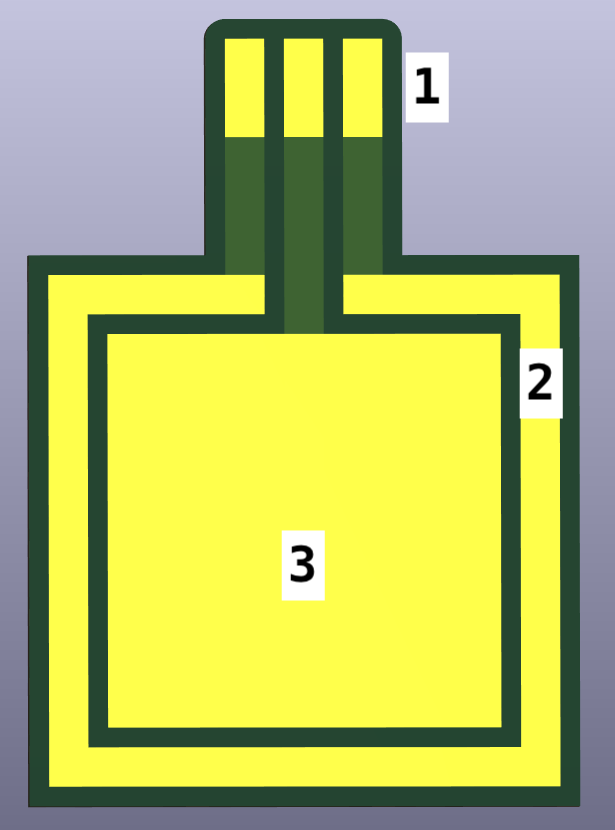
\includegraphics[width=0.3\textwidth]{Figures/GoldElectrode}
    \caption{The gold electrode \gls{pcb} design.}
    \label{fig:gold-electrode} %chktex 24
\end{figure}

The dimensions of the gold electrodes were chosen somewhat arbitrarily with the pads having a large area while being placed relatively close together to reduce the fringing but not too close to prevent water from flowing between the pads.
Additionally, the aim was to keep the resistance between the pads low to lower the amount of voltage required to generate a current through the water thus further reducing the fringing. 
The gold electrodes were designed with a $20mm \times 20mm$ pad area with a $2mm$ wide fringe guard surrounding the majority of the pad and the electrodes were spaced $10mm$ apart.
This gave a resistance from $3.75\Omega$ to $6.25\Omega$ between the gold electrodes for salinities from $40$ to $25$ on the Practical Salinity Scale PSS-78 respectively.

The titanium electrodes are substantially simpler and cheaper than the gold electrodes and would be the preferred electrodes if the fringing effect could be mathematically accounted and corrected for.
Provided the testing with the gold electrodes is able to prove a constant resistance-voltage relationship, the fringing effect between the titanium electrodes could be measured and accounted for allowing for them to be used as the primary electrodes in a future iteration of the device.
The titanium wire that was available for this project was $1mm$ in diameter and in order to account for the unknown resistance between the electrodes, the design allowed for an adjustable spacing between the electrodes and adjustable electrode length.

\section{Resistance Measurement Method}

The most common and practical method of measuring resistance is to use a resistor divider circuit which is what this project chose to use. 
The electrodes were chosen to be the $R_2$ resistor in the voltage divider and the $R_1$ resistor was chosen to be a significantly larger, known resistance.
This configuration had two advantages: it would reduce the voltage required to generate a current through the water and thus reduce the fringing effect, and it would prevent the board from being short-circuited if the electrodes were to touch as the $R_1$ resistor would limit the current.
The measurement taken from the voltage divider was then amplified using an op-amp to increase the resolution of the voltage measurement.

\section{Circuit Overview}

\begin{figure}
    \centering
    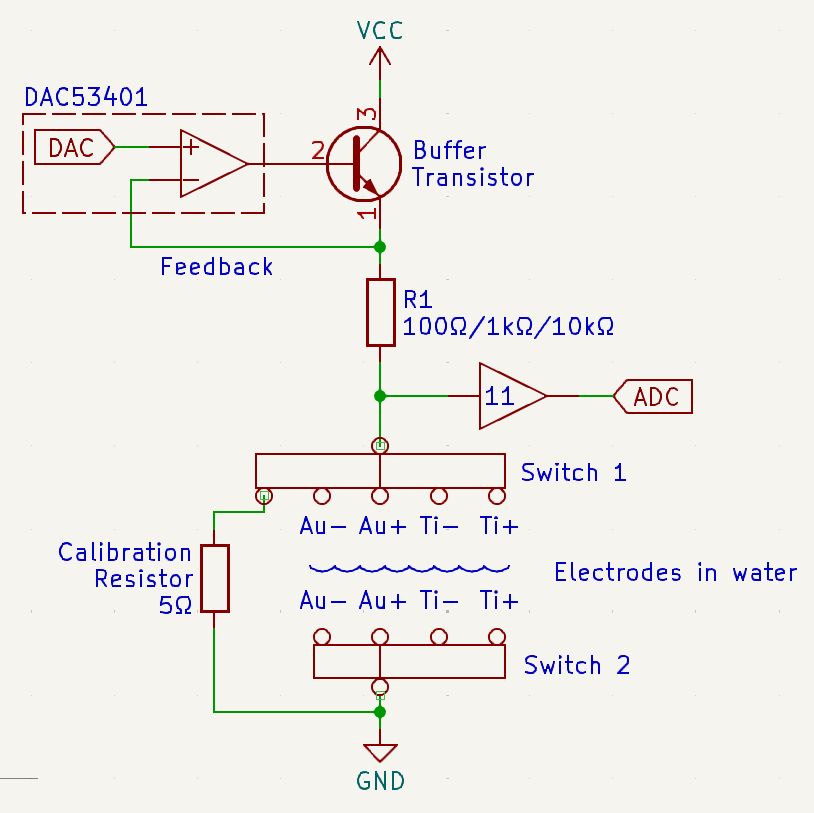
\includegraphics[width=0.6\textwidth]{Figures/CircuitOverview}
    \caption{A simplified representation of the resistance measuring circuit.}
    \label{fig:circuit-overview} %chktex 24
\end{figure}

\reffig{fig:circuit-overview} shows a simplified overview of the resistance measuring circuit that was used in this project. 
The circuit was designed to be printed onto a \gls{pcb} (herewith referred to as the probe) manufactured with \texttt{JLCPCB} due to their low cost, ease of manufacturing, precision relative to hand soldering and the familiarity of the author with the process.

The voltage driving the resistor divider was provided by a \gls{dac} such that the voltage could be varied and the resistance-voltage relationship could be determined of the salt water between the electrodes.
The \gls{dac} model was chosen from the available \glspl{dac} on the \texttt{JLCPCB} website and the DAC53401 was chosen for its high updated rate of $10us$, and it had advanced functionality allowing it to output square, triangle and sawtooth waves which would allow for high frequency tests.
The output \gls{dac} was then connected to a buffer transistor and the output of the buffer was connected to the feedback of the \gls{dac}.
This would allow a higher current to be drawn than what the \gls{dac} was rated for while still maintaining the desired output voltage.

The $R_1$ value that was chosen to pair with the gold electrodes was $100\Omega$ as it was the smallest e12 series resistance that would prevent the board from drawing too much current.
Due to the unknown resistance between the titanium electrodes, additional $R_1$ resistors were added to the board to allow for a range of resistance measurements.
Thus, the $R_1$ values were chosen to be $100\Omega$, $1k\Omega$ and $10k\Omega$ which would be used when the resistance between the probes is $1\Omega - 10\Omega$, $10\Omega - 100\Omega$ and $100\Omega - 1k\Omega$ respectively.
This would allow for a minimum resolution of $11\%$ of $V_{CC}$ for the voltage measurement by the \gls{adc} as shown by \refeqn{eqn:adc-resolution}.
\begin{align}\label{eqn:adc-resolution}
    \lfrac{1\Omega}{1\Omega + 100\Omega} * 11 = 11\% \\
    \lfrac{10\Omega}{10\Omega + 100\Omega} * 11 = 100\%
\end{align} 

Switch 1 allows $R_1$ to be connected to any of the four electrodes or the calibration resistor of $5\Omega$ and switch 2 allows for the other electrode to be connected to ground.
For example, switch 1 could be connected to Ti+ and switch 2 could be connected to Ti- to measure the resistance between the titanium electrodes.
This configuration also allows current to flow in both directions between electrodes which can prevent an excessive build up of chlorine gas or sodium electroplating on the electrodes by taking a resistance measurement in both directions in rapid succession.

In order to increase the measurement accuracy of the resistance, multiple high accuracy resistors were placed in series to attain the values of $R_1$ and the calibration resistor as this decreases the uncertainty of their resistance.
This total uncertainty of the parallel resistors $\delta_{R_{total}}$ is decreased by a factor equal to number of parallel resistors $n$ compared to each individual resistor's uncertainty $\delta_R$ as shown by \refeqn{eqn:parallel-resistor-total} to \refeqn{eqn:parallel-resistor-uncertainty}.
\begin{gather}
    R_{total} = {\left[ \sum_{i=1}^{n} \lfrac{1}{R} \right]}^{-1} = {\left(\lfrac{n}{R}\right)}^{-1} = \lfrac{1}{n}\cdot R \label{eqn:parallel-resistor-total} \\
    \text{for a function}~f(x_1,x_2,\dots,x_n),~\text{its tolerance} ~\delta_f = \sqrt{\sum_{i=1}^{n} {\left( \lfrac{\partial f}{\partial x_i} \delta x_i \right)}^2} \label{eqn:uncertainty-general-formula} \\
    \therefore \delta_{R_{total}} = \sqrt{{\left( \lfrac{\partial R_{total}}{\partial R} \delta_R \right)}^2} = \sqrt{{\left( \lfrac{1}{n} \delta_R \right)}^2} = \lfrac{1}{n} \delta_R \label{eqn:parallel-resistor-uncertainty}
\end{gather}
The resistances for $R_1$ were made from 3 parallel resistors with tolerance $\pm1\%$ giving a total tolerance of $\pm0.\bar{3}\%$ and the calibration resistor was made from 4 parallel resistors with tolerance $\pm1\%$ giving a total tolerance of $\pm0.25\%$.

\begin{figure}[!h]
    \centering
    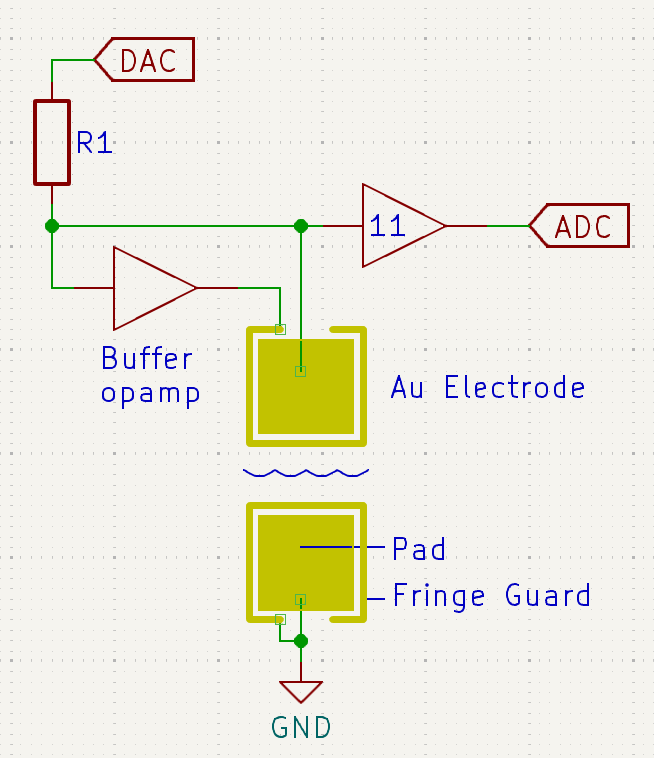
\includegraphics[width=0.4\textwidth]{Figures/AuElectrodeExample}
    \caption{A simplified representation of the resistance measurement circuit using the gold electrodes with the fringe guard.}
    \label{fig:au-measurement-circuit} %chktex 24
\end{figure}

\reffig{fig:au-measurement-circuit} shows an example switch configuration where the gold electrodes are used.
The voltage from the \gls{dac} is routed through the $R_1$ resistor and then through the gold electrodes pads as well as to a buffer op-amp which repeats the voltage through fringe guard without affecting the voltage between the main pads. 
A set of switches was also added to electrically disconnect the fringe guards to test for their effectiveness.
The fringe guards had the same voltage as the main pads with a lower conductivity so the current flowing between the fringe guards was assumed to be less than that of the pads and thus there was no need to limit the current from the op-amp.

\section{Salinity Calculation and Display}

In order to measure the salinity of the sea ice, the probe \gls{pcb} needed to be lowered into the water and measure salinity at various depths.
There are two methods for capturing the salinity data: either to constantly record the salinity data as the device it lowered through the water column or to have the device take a measurement when instructed by a controller.
The former method creates logistical problems with waterproofing the device and retrieving data while the latter was a more user-friendly approach allowing researchers to control exactly which depths the salinity is measured at and thus it was chosen for this project.

The controller was a basic \gls{pcb} with input buttons, input rotary switches, two 7-segment displays, an RS485 communication port and a simple microcontroller.
The RS485 communication port was chosen as the communication protocol as RS485 has the longest range and a high noise resistance which is necessary for the device to be used in the ocean which has high \gls{emi}.
The author was also familiar with the protocol and had previous board to board communication experience with it.
The microcontroller was arbitrarily chosen from the STM32F030 series as it was relatively cheap, it did not need to perform any complex calculations, and the author was familiar with the STM microcontroller series.

With an external controller, a waterproofed probe could be lowered into the water and measure the water's salinity.
The chosen method of waterproofing probe was to coat it with a layer of epoxy resin to waterproof it as this was the most familiar and cost-efficient method available.
In addition to the ports for the conductivity electrodes and the circuitry shown in \reffig{fig:circuit-overview}, the probe had temperature and depth sensors which are discussed in \refsec{sec:temp-depth-measurement}, an RS485 communication port and a microcontroller.
The microcontroller was chosen from the STM32F4 series as STM microcontrollers as they have a \gls{fpu} which allowed for the salinity calculation to be performed on the probe.

\section{Temperature and Depth Measurement}\label{sec:temp-depth-measurement}

Depth sensors that are waterproof are too expensive for this project's budget.
However, there have been alternative approaches which use non-waterproof sensors that are isolated form the water using a flexible membrane that would allow the pressure to be transmitted to the sensor. \textit{[citation needed]}
The depth sensor for this project was chosen as the cheapest depth that could handle above 50 meters of water pressure available at \texttt{JLCPCB} which was the WF183DE.
This project included a depth sensor with the aim to use this method to measure the depth of the probe in the water, however it also included a method for the user to manually input the depth of the probe in the water using the controller should this method fail.

The temperature sensor used in this project was an arbitrarily chosen, surface mount temperature sensor that had high accuracy and a wide temperature range.
The temperature sensor should be coated with a thin layer of epoxy resin to waterproof it as epoxy resin is a poor thermal conductor and thus a thinner layer would allow for a more accurate temperature measurement.
The choice of microcontroller and pressure sensor also provided this board with two alternative temperature sensors with less accurate, however they could be used in the event that the primary temperature sensor failed.

\section{PCB Assembly and Corrections}

\textit{TODO: pcb correction and labelled diagram.}

\section{Probe Code}

The major steps in measuring salinity are to measure the conductivity of the water between the electrodes, measure the temperature and pressure of the water and then calculate the salinity.
An overview of this process along with steps for each major measurement is shown in \reffig{fig:probe-code-flowchart}.

\begin{figure}[h]
    \centering
    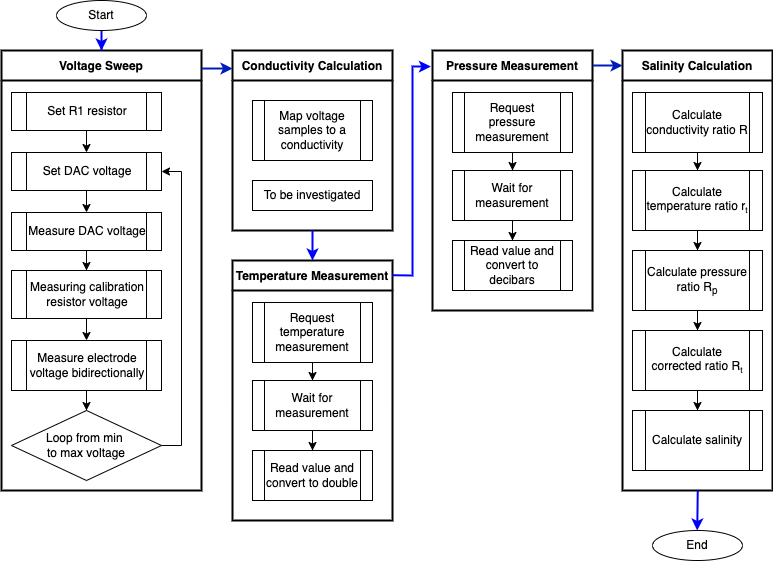
\includegraphics[width=1\textwidth]{Figures/probe_flowchart}
    \caption{The flowchart for the probe code that measures salinity.}
    \label{fig:probe-code-flowchart} %chktex 24
\end{figure}

The conductivity measurement and calculation is different depending on if the voltage-resistance relationship is constant or not which is expected for the gold and titanium electrodes respectively.
Both variations start with a voltage sweep where the voltage is increased from the minimum to the maximum voltage with a set voltage step or vice versa by the \gls{dac}.
At each step, the voltage output of the \gls{dac}, the voltage across the calibration resistor and the voltage across the electrodes are measured.

If the ratio between the \gls{dac} voltage and the voltage across the electrodes is not constant, the conductivity will have to be analysed by performing tests to create a model to relate each voltage sample to the conductivity of the water.

If the ratio between the \gls{dac} voltage and the voltage across the electrodes is constant, the resistance between the electrodes can be calculated using the calibration resistor.
Given that the calibration resistance and $R_1$ is known, the resistance between the electrodes can be calculated for each voltage sample using the ratio between the electrode and calibration voltages as shown in \refeqn{eqn:electrode-calib-resistance}.
$k$ is calculated using the known values $V_{ratio}$, $R_1$ and $R_{calibration}$ to simplify the equation as shown in \refeqn{eqn:electrode-calib-resistance-simplified} and finally $R_{electrode}$ can be calculated using \refeqn{eqn:electrode-calib-resistance-final}.
\begin{align}
    V_{ratio} &= \lfrac{V_{DAC}A_{11}A_{ADC}\lfrac{R_{electrode}}{R_1 + R_{electrode}}}{V_{DAC}A_{11}A_{ADC}\lfrac{R_{calibration}}{R_1 + R_{calibration}}} = \lfrac{\lfrac{R_{electrode}}{R_1 + R_{electrode}}}{\lfrac{R_{calibration}}{R_1 + R_{calibration}}} \label{eqn:electrode-calib-resistance} \\
    \lfrac{R_{electrode}}{R_1 + R_{electrode}} &= V_{ratio} \lfrac{R_{calibration}}{R_1 + R_{calibration}} = k \label{eqn:electrode-calib-resistance-simplified} \\
    R_{electrode} &= \lfrac{kR_1}{1 - k} \label{eqn:electrode-calib-resistance-final}
\end{align}
The resistance can then be averaged and the conductivity can be calculated for the gold electrodes using \refeqn{eqn:conductivity-from-resistance}.
Using this method allows for the device to nullify all scalar inaccuracies in the circuit including $R_1$ uncertainty, \gls{dac} and \gls{adc} gain errors, and the op-amp gain error as they will all be present in the calibration resistor and the electrodes measurements.
This method is however still vulnerable to offset inaccuracies including \gls{dac} and \gls{adc} offset errors and the internal resistance of the switches and traces.

Measuring the temperature and pressure is a simple matter of reading the temperature sensor and the pressure sensor respectively which finally allows salinity to be calculated which can be performed on the salinometer microcontroller as it possesses an \gls{fpu}.
Additionally, any of the temperature, depth, resistance or conductivity measurements can be calculated individually and transmitted to the controller if requested.

\section{Controller Code}

\textit{todo}

The controller's primary goal is to request measurements and display the returned values to the user.
However, once the probe is cast in epoxy resin it will become unprogrammable and thus the controller must also be able to configure the probe's settings.
The parameters that the controller will need to adjust include the $R_1$ resistance, the electrode type, whether to use the fringe shield or not, the voltage sweep range and steps and the number of \gls{adc} samples to average.